\documentclass{beamer} %
\usepackage[utf8]{inputenc}
\usepackage{amsmath,bm,bbm} 
\usepackage{amsthm,amsfonts,amssymb}
\usepackage{outlines}
\usepackage{times}
\usepackage{tikz}
\usepackage{amsmath}
\usepackage{verbatim}
\usepackage{graphicx}
\usepackage{tabularx}
\usepackage{siunitx}
\usepackage{enumitem}
\usepackage{booktabs}
\usetheme{CambridgeUS}
\usefonttheme{professionalfonts}
\usetikzlibrary{arrows,shapes}


\title[Séries Temporais]{Otimização de Algoritmos de Análise de Séries Temporais Utilizando a Interface .Call()}
\author{Roger Almeida$^{1}$ Alejandro C.\ Frery$^{2}$}

\institute{$^{1}$UFAL - Bacharelado em Engenharia da Computação\\
$^{2}$UFAL - Laboratório de Computação Científica e Análise Numérica}

\date{02 de abril de 2019}

\AtBeginSection[]
{
  \begin{frame}<beamer>
    \frametitle{Sumário}
    \tableofcontents[currentsection,currentsubsection]
  \end{frame}
}

\begin{document}

\maketitle


% For every picture that defines or uses external nodes, you'll have to
% apply the 'remember picture' style. To avoid some typing, we'll apply
% the style to all pictures.
\tikzstyle{every picture}+=[remember picture]

% By default all math in TikZ nodes are set in inline mode. Change this to
% displaystyle so that we don't get small fractions.
\everymath{\displaystyle}

% Uncomment these lines for an automatically generated outline.
\begin{frame}{Sumário}
  \tableofcontents
\end{frame}

\section{Séries Temporais e Teoria da Informação}

\begin{frame}{Séries Temporais}

Tratam-se de conjuntos de dados, obtidos por meio de um processo observacional
ao longo de um determinado período de tempo.

\vspace{0.8cm}

\textbf{Etapas do processo de análise}

\begin{itemize}
    \item \textbf{Simbolização}
    \begin{itemize}
        \item Processo de simbolização de Bandt e Pompe\cite{bandt2002permutation}
    \end{itemize}
    \vspace{0.5cm}
    \item \textbf{Extração de informações}
    \begin{itemize}
        \item Entropias
        \item Distâncias estocásticas
        \item Complexidade estatística
    \end{itemize}
\end{itemize}

\end{frame}

\begin{frame}{A Simbolização de Bandt \& Pompe}

Dada uma série temporal $\bm {X_t} = (x_1, x_2, \dots, x_N)$ e uma dimensão $D$. Dividimos a série temporal em padrões de dimensão $D$, onde seus valores serão ordenados e simbolizados de acordo com seu índice.\\
\vspace{0.3cm}
Por exemplo, seja $\chi = (4,3,9,10,6)$ uma série temporal, e considerando $D$ = 4 a dimensão, então obteremos dois padrões:\\
\begin{itemize}
    \item$\pi_1 = 2134$, pois $x_2 < x_1 < x_3 < x_4$,
    \item$\pi_2 = 1423$, pois $x_1 < x_4 < x_2 < x_1$.
\end{itemize}
 
\end{frame}

\begin{frame}{Distribuição de probabilidade e Teoria da Informação}

Através da simbolização de Bandt \& Pompe podemos extrair a distribuição de probabilidade $p(\pi)$ das $D!$ permutações $\pi$. $p(\pi)$ é dada por:


\begin{itemize}
    \item $p(\pi) = \frac{\# \left\{t| t \leq N - D, (x_1,\dots,x_N)  \hbox{has type} \pi\right\}}{N - D + 1}$.\\
\end{itemize}


E com isso podemos utilizar os descritores da teoria da informação para extrair informações sobre nosso sistema, como a entropia, a distância estocástica e a complexidade estatística.

\end{frame}

\section{Imputação de dados}

\begin{frame}{Qual é o problema?}

Ao introduzirem a ideia de entropia de permutação e o método de simbolização, Bandt \& Pompe assumiram como condição inicial que os dados analisados consistiam em valores contínuos, ou seja, que na série temporal a ser analisada não existe $x_i = x_j$, onde $i \neq j$. Mas e se trabalharmos com dados discretos o que acontece se houverem repetições?

\end{frame}

\begin{frame}{Solução}

Diversas estratégias eficazes foram apresentadas para contornar o problema da repetição de dados, trabalhamos com quatro delas:

\begin{itemize}
    \item \textbf{Complete Case Imputation}
    \item \textbf{Time Ordered Imputation}
    \item \textbf{Random Imputation}
    \item \textbf{Data Driven Imputation}\cite{traversaro2018bandt}
\end{itemize}

\end{frame}

\begin{frame}{Algoritmos de Imputação de Dados}

\begin{itemize}
    \item \textbf{Complete Case Imputation}\\
    Elimina todos os padrões que contém elementos repetidos do cálculo da probabilidade.
    \item \textbf{Time Ordered Imputation}\\
    Se $x_{t1} = x_{t2}$ e $t_{1} < t_{2}$ então $x_{t1} < x_{t2}$.
    \item \textbf{Random Imputation}\\
    Adiciona-se à probabilidade de cada padrão um peso probabilístico baseado na quantidade de elementos repetidos do padrão.
    \item \textbf{Data Driven Imputation}\\
    Adiciona-se à probabilidade de cada padrão uma perturbação extraída de uma distribuição de probabilidade calculada previamente através do método Complete Case.
\end{itemize}
    
\end{frame}

\section{.Call() na otimização dos algoritmos de imputação de dados}

\begin{frame}{Qual o problema?}

Os algoritmos em R anteriormente criados para a imputação de padrões de séries temporais se mostraram eficazes e precisos em seus resultados. Porém, tendo em vista que era necessária a análise de diversas séries temporais de tamanho muito grande, os algoritmos possuíam um tempo de execução inviável. Com isso veio a necessidade de um meio de incrementar a velocidade desses algoritmos.
    
\end{frame}

\begin{frame}{Solução}
    
Uma solução encontrada para o problema da velocidade foi a utilização da interface \textit{.Call()}\cite{Speed}, que funciona como uma ponte entre as duas linguagens, possibilitando “chamar” funções escritas em C dentro de um código em R, e assim transmitindo dados entre as duas plataformas.
    
\end{frame}

\begin{frame}{Implementação}
 As seguintes bibliotecas devem ser incluídas: \textit{R.h, Rinternals.h, Rmath.h}. \\
 \vspace{0.3cm}
 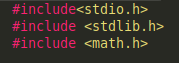
\includegraphics[width=0.25\columnwidth]{include.png}\\
 
 A função em C é declarada como retornando um tipo \textbf{SEXP}, que significa \textit{Simple EXPression}, todos os dados divididos entre as duas linguagens precisam ser deste tipo, ou seja, todos os dados recebidos pela função em C são desta forma e o array de distribuição de probabilidade criado pela função também assume esse tipo.\cite{.Call,Extensions}
 \vspace{0.3cm}
 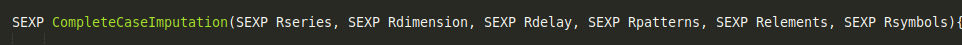
\includegraphics[width=01.00\columnwidth]{chamada.png}\\
     
\end{frame}

\begin{frame}{Implementação}
O arquivo .c deve ser compilado com o comando \textit{R CMD SHLIB arquivo.c}, isso gerará um novo arquivo do tipo \textit{.so}.
\vspace{0.3cm}    
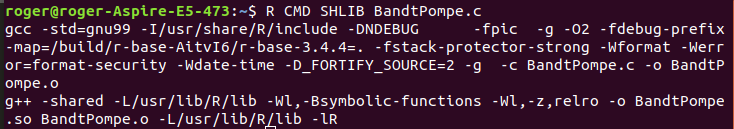
\includegraphics[width=0.80\columnwidth]{terminal.png}\\
\vspace{0.3cm}
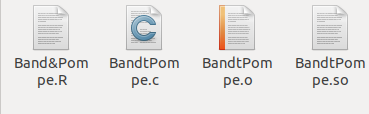
\includegraphics[width=0.50\columnwidth]{arquivos.png}\\
\vspace{0.3cm}
\end{frame}

\begin{frame}{Implementação}

 No programa em R, esse arquivo \textit{.so} deve ser carregado através do comando \textit{dyn.load(arquivo.so)}, em seguida se pode utilizar a função em C através da interface utilizada com \textit{.Call(função, ...)}, onde após o nome da função são inseridos todos os parâmetros necessários.\\

\begin{figure}[h]
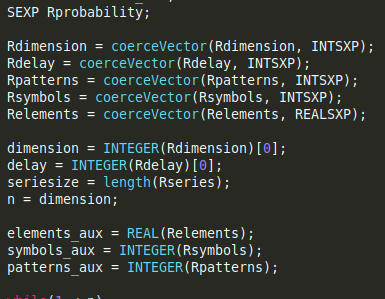
\includegraphics[scale=0.25]{conversao.png}
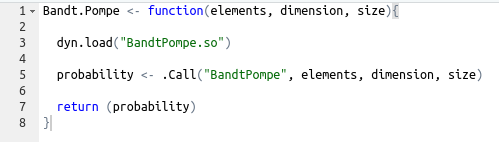
\includegraphics[scale=0.35]{BP.png}
\end{figure}
\end{frame}

\begin{frame}{Resultados}

A velocidade do algoritmo original em R foi comparada com a do algoritmo utilizando C. Os algoritmos implementados e analisados até o momento foram o Complete Case e o Time Ordered. Para calcular o tempo de execução de cada uma foi utilizado o seguinte algoritmo:
    
\begin{flushleft}
\textit{start.time $<$- Sys.time()\\
--- função a ser analisada ---\\
end.time $<$- Sys.time()\\
time.taken $<$- end.time - start.time\\}
\end{flushleft}

Onde a variável time.taken nos diz exatamente o tempo levado para executar a função testada.
    
\end{frame}

\begin{frame}{Resultados}
    
Abaixo segue uma tabela, baseada numa amostra obtida a partir de dez distintas execuções dos programas, comparando os tempos de execução das implementações do Complete Case em cada linguagem:\\
\vspace{0.3cm}

\begin{tabular}{|c|c|c|c|}
     \hline
      & Valor mínimo & Valor máximo & Média\\
      \hline
      R & \SI{31.67778}{\second} & \SI{34.97058}{\second} & \SI{33.05312}{\second}\\
      \hline
      C & \SI{0.321858}{\second} & \SI{0.3651605}{\second} & \SI{0.3360521}{\second}\\
      \hline
\end{tabular}\\
\vspace{0.3cm}

Ou seja, tendo como base a média de tempo, é fácil ver que a versão em C é aproximadamente cem vezes mais veloz que a versão em R.
    
\end{frame}

\begin{frame}{Resultados}
    
Quanto à implementação da Time Ordered, analisando também sua velocidade em ambas as versões, com o mesmo número de amostragem, obtém-se a seguinte tabela:\\

\vspace{0.3cm}
\begin{tabular}{|c|c|c|c|}
     \hline
      & Valor mínimo & Valor máximo & Média\\
      \hline
      R & \SI{129.3993}{\second} & \SI{142.9892}{\second} & \SI{135.4226}{\second}\\
      \hline
      C & \SI{1.806375}{\second} & \SI{1.903321}{\second} & \SI{1.849567}{\second}\\
      \hline
\end{tabular}\\
\vspace{0.3cm}
Tal qual o Complete Case, vemos que a velocidade da versão em C do Time Ordered supera em muito a versão em R.
    
\end{frame}

\begin{frame}{Conclusão}
    
Com isto, temos que os algoritmos sendo desenvolvidos em C serão mais vantajosos, pois possuem a mesma precisão mas com superior velocidade, o que facilitará suas aplicações no futuro.

\end{frame}

\begin{frame}{Referências}
    \bibliographystyle{abbrv}
    \tiny\bibliography{ref.bib}
\end{frame}

\end{document}